% arara: pdflatex
% arara: pdflatex
\documentclass[journal]{IEEEtran}
\usepackage{graphicx}
\usepackage{	array,
			cite,
			graphicx,
			mathtools
			}
\usepackage{soul}
\usepackage{/Users/aviatorblue/Documents/mcode}
\graphicspath{ {./images/} } % Graphics Path



\begin{document}

\title{Direct Sequence-Spread Spectrum}
\author{David M Houston\\
		Oregon Institute of Technology\\\\
		}
\date{April 21, 2015}

\maketitle

\begin{abstract}
This project explained the ideas encompassing Direct Sequence-Spread Spectrum as it relates to RF communication systems and a discussion of Code-Division Multiple Access (CDMA). This was done using mathematical models of physical systems to conceptual complex ideas and bring them down to realistic outcomes and measurable outputs.
\end{abstract}

\section{Introduction}
Direct Sequence-Spread Spectrum is a communication type which takes a digital I/O signal of information and modulates it with a pseudorandom binary sequence. This allows it to go under a significant amount of noise without a loss of data transfer to the receiver due to the signal riding on a noise signal. This allows the user to transmit in a very noisy environment where the noise floor is far above the expected thermal noise floor, or the KTB, an allows encryption of the data which is very secure based on the repetition of the pseudo-binary random number (PN). This form of communication can be used in combination with Bilateral Phase-Shift Keying (BPSK), CDMA, and frequency hopping and is utilized in GPS, Wifi, and various secure communication arrays. 

\section{Background}
WARNING: JUST A PLACE HOLDER
In telecommunications, direct-sequence spread spectrum (DSSS) is a spread spectrum modulation technique. Spread spectrum systems are such that they transmit the message bearing signals using a bandwidth that is in excess of the bandwidth that is actually needed by the message signal. One of the methods of achieving this spreading of the message signal is provided by DSSS modulation. In DSSS the message signal is used to modulate a bit sequence known as the Pseudo Noise (PN) code; this PN code consists of pulses of a much shorter duration (larger bandwidth) than the pulse duration of the message signal, therefore the modulation by the message signal has the effect of chopping up the pulses of the message signal and thereby resulting in a signal which has a bandwidth nearly as large as that of the PN sequence.[1] In this context the duration of the pulse of the PN code is referred to as the chip duration and the smaller this value, the larger the bandwidth of the resultant DSSS signal and the more immune to interference the resultant signal becomes.[1] Some of the uses of DSSS include the Code Division Multiple Access (CDMA) channel access method and the IEEE 802.11b specification used in Wi-Fi networks.[2][3]

\section{Signal Creation}
Spread spectrum is first created by a PN and a data signal. The data signal is a string of character created into an array of 8 bit binary number combinations based on the ASCII value of the characters. This gives our signal length as well some complexity for accurate transition analysis. This is fed through an encoder which converts a signal bit into 16 bits of that same value. This is used for voting to reduce bit error. This signal has a frequency spectrum which matches the following graphs (see Figure~\ref{fig:id}). Usually it is preferred that a digital I/O signal is modulated by a PN whose bit rate is much higher than the digital I/O signals bit rate. This PN signal has a frequency spectrum which is very noisy containing all of the frequencies, just like white noise (see Figure~\ref{fig:PN}).\\

\begin{figure}[h!]
\centering
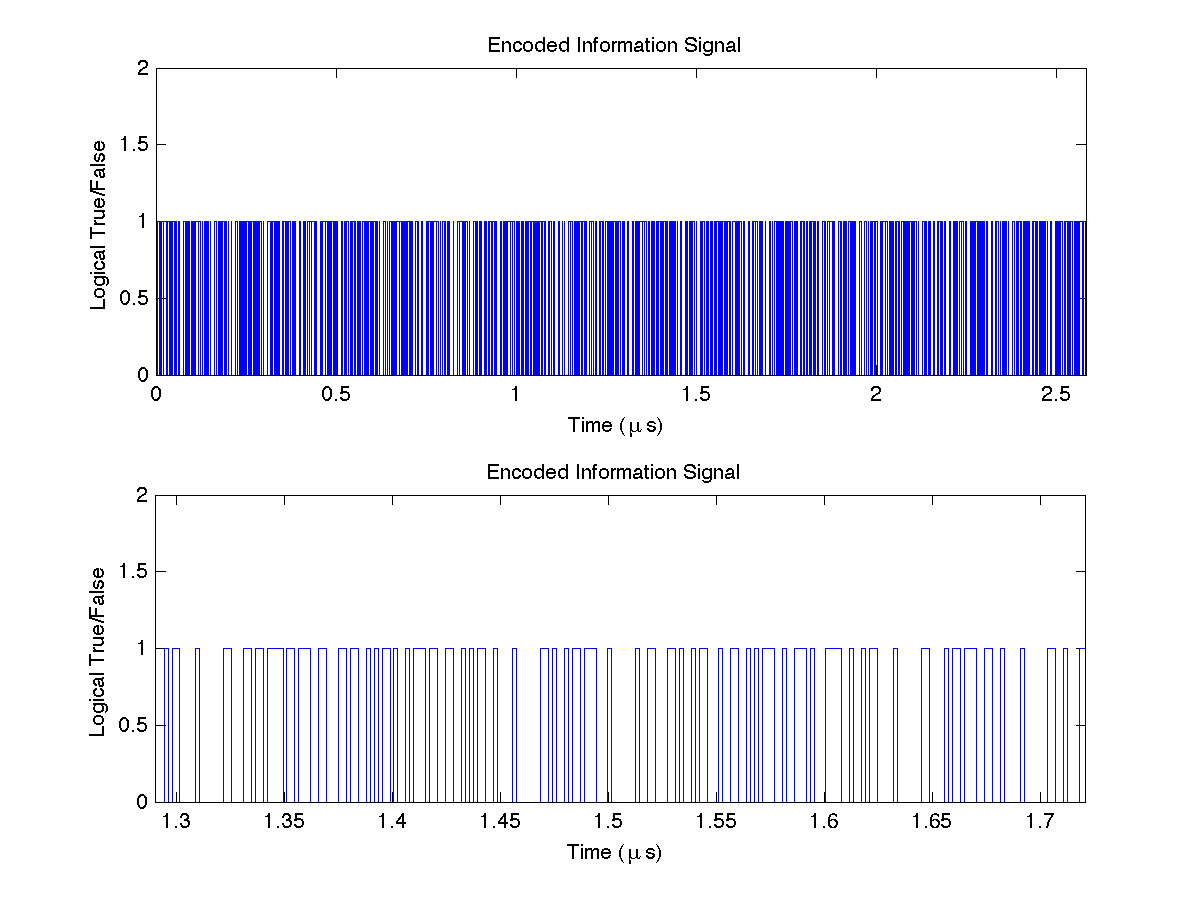
\includegraphics[width=3in]{encoded_signal.png}
\caption{Digital I/O Encoded Signal}
\label{fig:dio}
\end{figure}

\begin{figure}[h!]
\centering
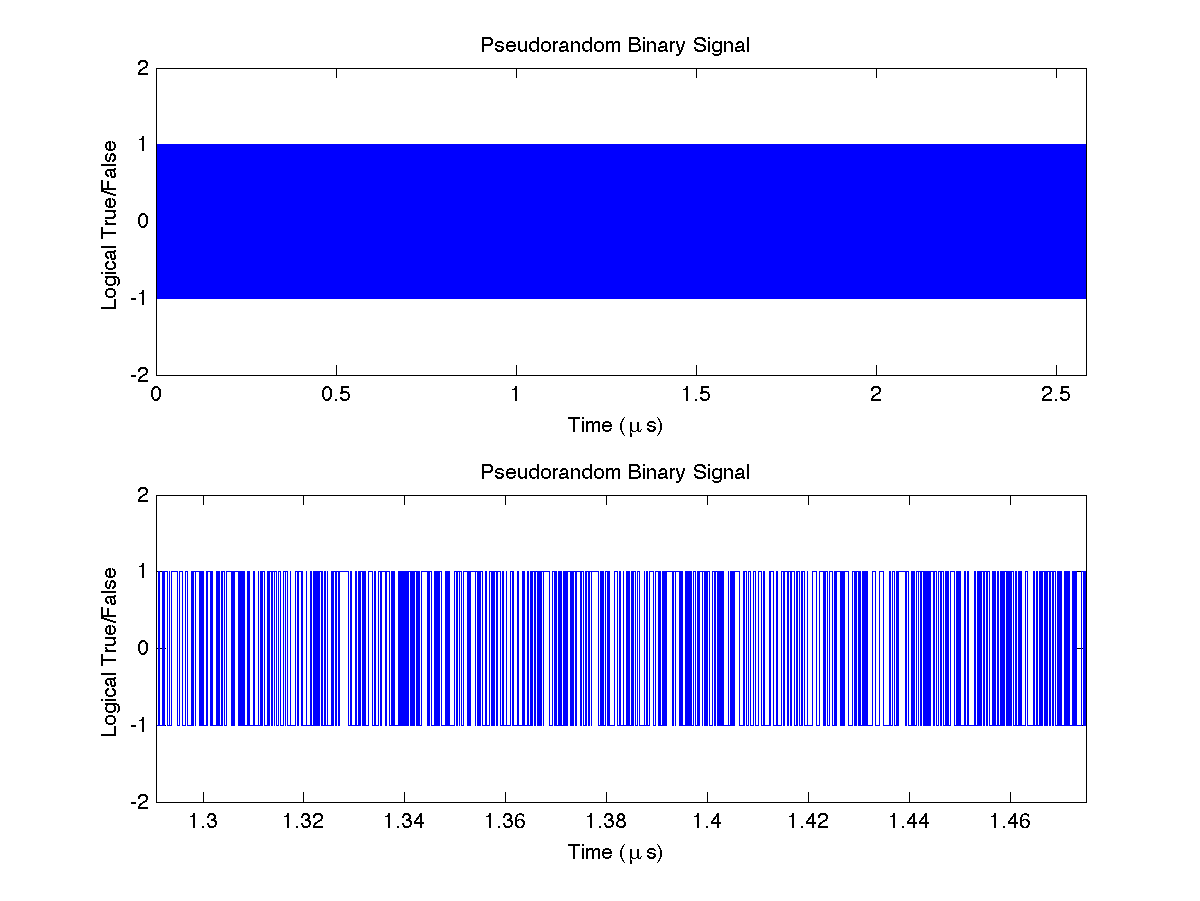
\includegraphics[width=3in]{pseudo_signal.png}
\caption{PN Signal}
\label{fig:PN}
\end{figure}
\end{appendices}

These two signals are then modulated together to form a digital I/O signal carried by a PN signal creating the basis for the DSSS signal (see Figure~\ref{fig:mod_PN}). This signal is then band limited and carrier by a Large Carrier signal (see Figure~\ref{fig:dsb_lc}) which can be demodulated by the receiver and then down converted. In order to reduce the bit transfer error of this form of communication the frequency of the PN was decreased to eliminate losses with the band limiting of the signal. When the signal was band limited a bit error of $\~13\%$ was observed. However, when the signal was transmitted on a carrier and then demodulated using a synchronous demodulator only a $0.25\%$ increase in bit loss was observed, after applying an amplifier to boost the signal.

\begin{figure}[h!]
\centering
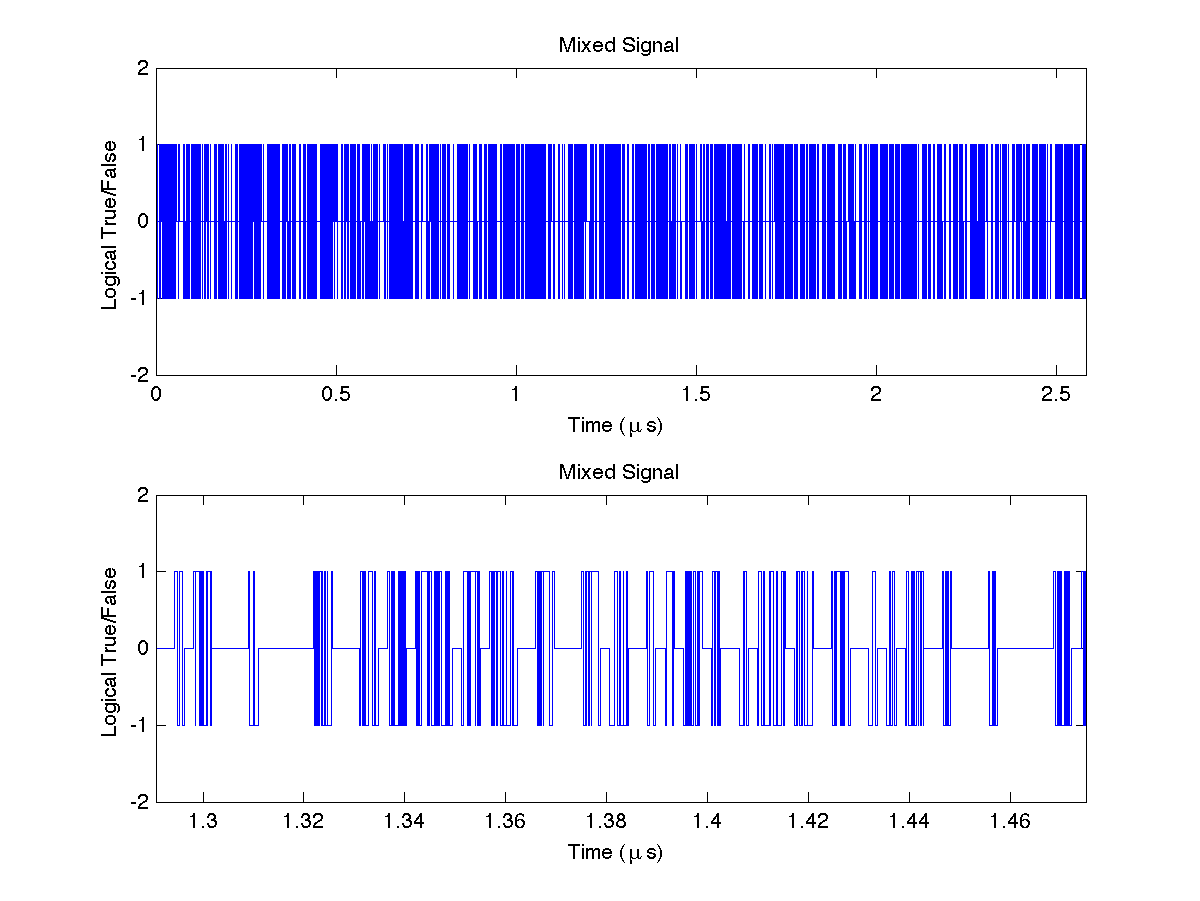
\includegraphics[width=3in]{dsss.png}
\caption{Modulated PN-Digital I/O Signal}
\label{fig:mod_PN}
\end{figure}

\begin{figure}[h!]
\centering
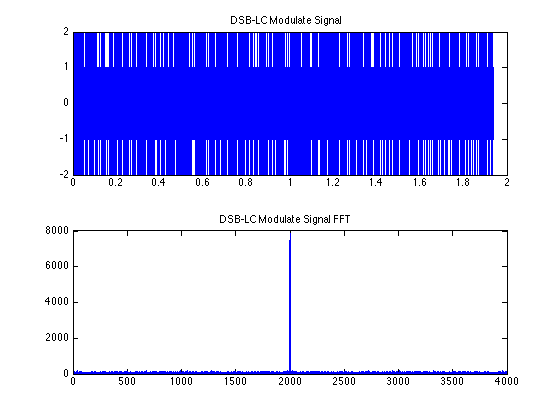
\includegraphics[width=3in]{dsb_lc.png}
\caption{DSB-LC Signal}
\label{fig:dsb_lc}
\end{figure}

This signal is then despread to recreate the original signal. This despreading is done by multiplying the demodulating signal by the original PN (see Figure~\ref{fig:despread}). To verify the signals integrity a comparison was done to compare the bit error of the signal and it was found to have $\~13.25\%$ bit error. This error, as discussed above, is due to the band limiting of the signal for transmutation. HT

\begin{figure}
\centering
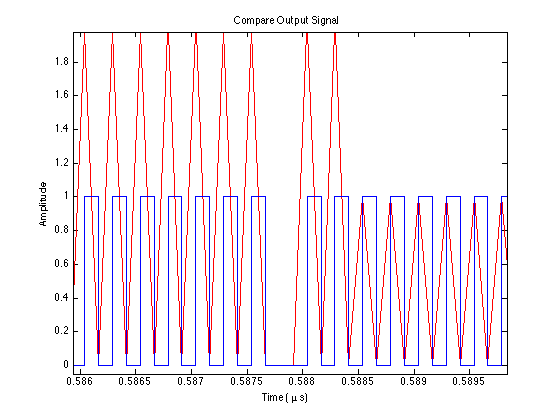
\includegraphics[width=3in]{despread.png}
\caption{DSB-LC Signal}
\label{fig:despread}
\end{figure}

\section{White Noise}
When a signal accomponies additive white gaussian noise (AWGN) the signal to noise ratio decreases rapidly, however, for DSSS the result is quite the opposite. 


\end{document}
